\documentclass[aspectratio=169,11pt]{beamer}
\usetheme{Boadilla}
\usecolortheme{seahorse}
\usepackage{listings}
\usepackage{tikz}
\tikzset{ast/.style={every node/.style={draw=codeblue,rounded corners=2pt,fill=blue!4,inner sep=5pt,font=\small},edge from parent/.style={draw=codeblue,thick},level distance=1cm,sibling distance=2cm}, astlabel/.style={draw=none,fill=none,font=\scriptsize,text=black,inner sep=2pt}}
\usepackage{amsmath,amssymb,booktabs}
\definecolor{codeblue}{RGB}{25,65,125}
\setbeamertemplate{navigation symbols}{}
\setbeamertemplate{footline}[frame number]
\setbeamercolor{structure}{fg=codeblue}
\lstset{language=Python,basicstyle=\ttfamily\small,keywordstyle=\color{codeblue}\bfseries,commentstyle=\color{gray},stringstyle=\color{teal},showstringspaces=false,columns=fullflexible,keepspaces=true,breaklines=true,tabsize=4}
\newcommand{\FV}{\operatorname{FV}}
\newcommand{\sz}{\operatorname{size}}
\title{Lambda Calculus in Python}
\subtitle{Reading \texttt{lambda0.py}}
\author{CS413}
\date{September 8, 2026}
\begin{document}
\begin{frame}\titlepage\end{frame}

\begin{frame}{The language represented by the code}
An untyped lambda term has one of three forms:
\[
M,N ::= x \quad\mid\quad \lambda x.M \quad\mid\quad M\,N
\]
\begin{center}
\begin{tabular}{lll}\toprule
Form & Meaning & Python constructor\\\midrule
$x$ & Variable & \texttt{T0Mvar(x)}\\
$\lambda x.M$ & Abstraction & \texttt{T0Mlam(x, M)}\\
$M\,N$ & Application & \texttt{T0Mapp(M, N)}\\\bottomrule
\end{tabular}
\end{center}
\medskip
Each constructor builds a node in an abstract syntax tree.\\
Constructing an application does not evaluate it.
\end{frame}

\begin{frame}[fragile]{The common base class and type aliases}
\begin{lstlisting}
type sint = int
type strn = str

@dataclass
class T0M000(ABC):
    ctag = "T0M000"
    pass

type t0erm = T0M000
\end{lstlisting}
\begin{itemize}
\item The aliases give familiar Python types names used in this file.
\item All term constructors inherit from \texttt{T0M000}.
\item \texttt{ABC} alone does not prevent instantiation: there are no abstract methods.
\item The \texttt{type} alias syntax requires Python 3.12 or later.
\end{itemize}
\end{frame}

\begin{frame}[fragile]{Data classes encode the three term forms}
\begin{columns}[T]
\begin{column}{0.49\textwidth}
\begin{lstlisting}
@dataclass
class T0Mvar(T0M000):
    arg1: strn
    ctag = "T0Mvar"

@dataclass
class T0Mlam(T0M000):
    arg1: strn
    arg2: t0erm
    ctag = "T0Mlam"
\end{lstlisting}
\end{column}
\begin{column}{0.49\textwidth}
\begin{lstlisting}
@dataclass
class T0Mapp(T0M000):
    arg1: t0erm
    arg2: t0erm
    ctag = "T0Mapp"
\end{lstlisting}
\medskip
\texttt{@dataclass} generates initialization, a printable representation, and equality.\\[0.7em]
\texttt{ctag} is a class attribute. The functions dispatch with \texttt{isinstance}, not with \texttt{ctag}.
\end{column}
\end{columns}
\end{frame}

\begin{frame}[fragile]{Reading a nested constructor expression}
\[
\lambda x.\,x\,y
\]
\begin{lstlisting}
T0Mlam("x",
    T0Mapp(
        T0Mvar("x"),
        T0Mvar("y")
    )
)
\end{lstlisting}
\begin{itemize}
\item The outer node binds the name \texttt{"x"} in its body.
\item The body is an application with two variable children.
\item The occurrence of $x$ is bound. The occurrence of $y$ is free.
\end{itemize}
Variable nodes store names. The surrounding lambdas determine binding.
\end{frame}

\begin{frame}[fragile]{The examples: I, K, and S}
\begin{align*}
I &= \lambda x.x\\
K &= \lambda x.\lambda y.x\\
S &= \lambda x.\lambda y.\lambda z.(x\,z)\,(y\,z)
\end{align*}
\begin{lstlisting}
EX_I = T0Mlam("x", T0Mvar("x"))
EX_K = T0Mlam("x", T0Mlam("y", T0Mvar("x")))
EX_S = T0Mlam("x", T0Mlam("y", T0Mlam("z",
    T0Mapp(
        T0Mapp(T0Mvar("x"), T0Mvar("z")),
        T0Mapp(T0Mvar("y"), T0Mvar("z"))
    ))))
\end{lstlisting}
The file builds and prints these terms. Line breaks above improve readability.
\end{frame}


\begin{frame}{AST nodes and their children}
\begin{columns}[T]
\begin{column}{.30\textwidth}\centering
\textbf{Variable: $x$}\\[1em]
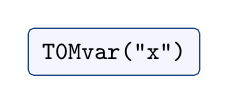
\begin{tikzpicture}[ast]
\node {\texttt{T0Mvar("x")}};
\end{tikzpicture}\\[1em]
A leaf has no children.\\[.6em]
\texttt{arg1} stores the name.
\end{column}
\begin{column}{.33\textwidth}\centering
\textbf{Abstraction: $\lambda x.M$}\\[1em]
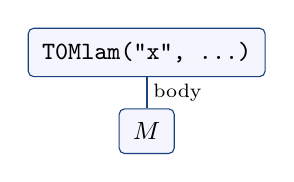
\begin{tikzpicture}[ast]
\node {\texttt{T0Mlam("x", ...)}}
 child {node {$M$} edge from parent node[astlabel,right] {body}};
\end{tikzpicture}\\[1em]
\texttt{arg1} stores the binder.\\[.6em]
\texttt{arg2} is the body child.
\end{column}
\begin{column}{.33\textwidth}\centering
\textbf{Application: $M\,N$}\\[1em]
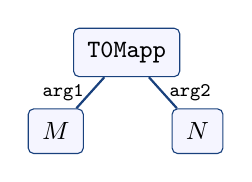
\begin{tikzpicture}[ast,sibling distance=1.8cm]
\node {\texttt{T0Mapp}}
 child {node {$M$} edge from parent node[astlabel,left] {\texttt{arg1}}}
 child {node {$N$} edge from parent node[astlabel,right] {\texttt{arg2}}};
\end{tikzpicture}\\[1em]
Left child: function.\\[.6em]
Right child: argument.
\end{column}
\end{columns}
\vfill
The next trees abbreviate the labels as $\lambda x$, $\mathsf{app}$, and $x$. Each drawn node represents one term object.
\end{frame}

\begin{frame}{The ASTs of I and K}
\begin{columns}[T]
\begin{column}{.48\textwidth}\centering
$I=\lambda x.x$\\[1em]
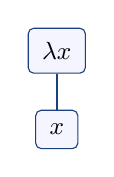
\begin{tikzpicture}[ast]
\node {$\lambda x$} child {node {$x$}};
\end{tikzpicture}\\[1em]
2 nodes: one lambda and one variable.\\[.6em]
The lambda binds the leaf $x$.
\end{column}
\begin{column}{.48\textwidth}\centering
$K=\lambda x.\lambda y.x$\\[1em]
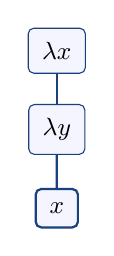
\begin{tikzpicture}[ast]
\node {$\lambda x$} child {node {$\lambda y$} child {node {$x$}}};
\end{tikzpicture}\\[1em]
3 nodes: two lambdas and one variable.\\[.6em]
The inner lambda has no occurrence of $y$.
\end{column}
\end{columns}
\vfill
The names on lambda nodes are fields, not extra variable leaves.
\end{frame}

\begin{frame}{The AST of S}
\begin{columns}[c]
\begin{column}{.52\textwidth}\centering
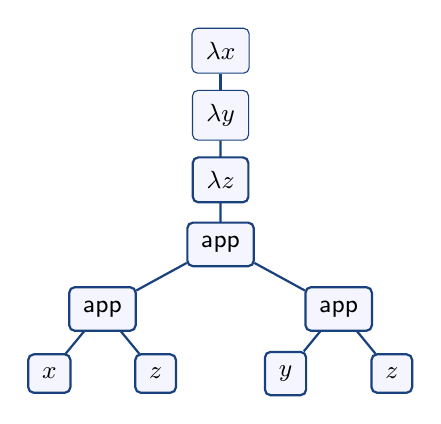
\begin{tikzpicture}[ast,level distance=.82cm,level 4/.style={sibling distance=3cm},level 5/.style={sibling distance=1.35cm}]
\node {$\lambda x$}
 child {node {$\lambda y$}
 child {node {$\lambda z$}
 child {node {$\mathsf{app}$}
 child {node {$\mathsf{app}$} child {node {$x$}} child {node {$z$}}}
 child {node {$\mathsf{app}$} child {node {$y$}} child {node {$z$}}}}}};
\end{tikzpicture}
\end{column}
\begin{column}{.46\textwidth}
$S=\lambda x.\lambda y.\lambda z.(x\,z)\,(y\,z)$\\[1.2em]
The outer application has two application subtrees:
\begin{itemize}
\item Left: $x\,z$
\item Right: $y\,z$
\end{itemize}
\medskip
$3$ lambdas $+\;3$ applications\\
$+\;4$ variable leaves $=\;10$ nodes.\\[1em]
The two $z$ leaves are separate occurrences of the same bound name.
\end{column}
\end{columns}
\end{frame}

\begin{frame}{Application grouping changes the tree}
\begin{columns}[T]
\begin{column}{.48\textwidth}\centering
$(x\,y)\,z$\\[1em]
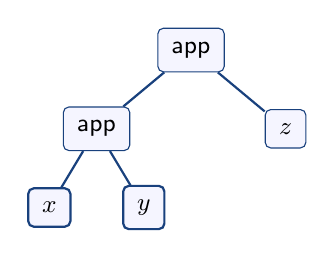
\begin{tikzpicture}[ast,sibling distance=2.4cm,level 2/.style={sibling distance=1.2cm}]
\node {$\mathsf{app}$}
 child {node {$\mathsf{app}$} child {node {$x$}} child {node {$y$}}}
 child {node {$z$}};
\end{tikzpicture}\\[1em]
The function child is an application.
\end{column}
\begin{column}{.48\textwidth}\centering
$x\,(y\,z)$\\[1em]
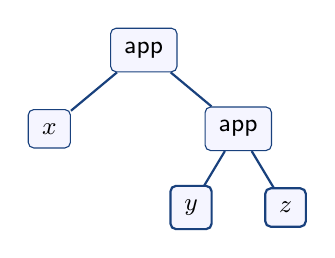
\begin{tikzpicture}[ast,sibling distance=2.4cm,level 2/.style={sibling distance=1.2cm}]
\node {$\mathsf{app}$}
 child {node {$x$}}
 child {node {$\mathsf{app}$} child {node {$y$}} child {node {$z$}}};
\end{tikzpicture}\\[1em]
The argument child is an application.
\end{column}
\end{columns}
\vfill
By convention, $x\,y\,z$ means $(x\,y)\,z$. Both trees have size $5$, but their structure differs.
\end{frame}

\begin{frame}{Binding scope in an AST}
\begin{columns}[c]
\begin{column}{.47\textwidth}\centering
$\lambda x.x\,y$\\[1em]
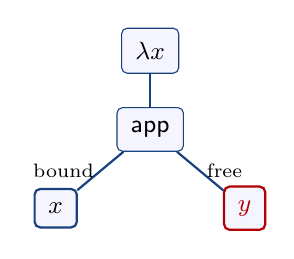
\begin{tikzpicture}[ast,sibling distance=2.4cm]
\node {$\lambda x$}
 child {node {$\mathsf{app}$}
 child {node {$x$} edge from parent node[astlabel,left] {bound}}
 child {node[draw=red!70!black,text=red!70!black] {$y$} edge from parent node[astlabel,right] {free}}};
\end{tikzpicture}
\end{column}
\begin{column}{.49\textwidth}
To classify a variable occurrence, walk toward the root.\\[1em]
The nearest lambda with the same name binds that occurrence. If none exists, the occurrence is free.\\[1em]
Here, $\FV(\lambda x.x\,y)=\{y\}$.\\[1em]
The drawn edges show syntax children. Binding comes from names and scope.
\end{column}
\end{columns}
\end{frame}

\begin{frame}{Shadowing: the nearest matching binder}
\begin{columns}[c]
\begin{column}{.49\textwidth}\centering
$\lambda x.x\,(\lambda x.x)$\\[1em]
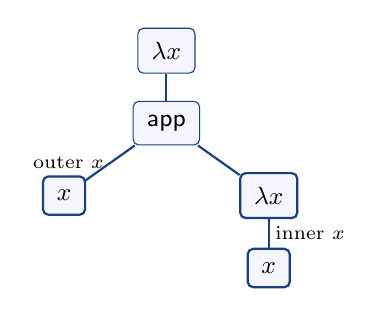
\begin{tikzpicture}[ast,sibling distance=2.6cm,level distance=.92cm]
\node {$\lambda x$}
 child {node {$\mathsf{app}$}
 child {node {$x$} edge from parent node[astlabel,left] {outer $x$}}
 child {node {$\lambda x$} child {node {$x$} edge from parent node[astlabel,right] {inner $x$}}}};
\end{tikzpicture}
\end{column}
\begin{column}{.47\textwidth}
The left leaf belongs to the outer binder.\\[1em]
The rightmost leaf belongs to the inner binder, which shadows the outer name.\\[1em]
Renaming only the inner binder and its occurrence gives an alpha-equivalent term:
\[
\lambda x.x\,(\lambda z.z)
\]
Both terms are closed and have size $5$.
\end{column}
\end{columns}
\end{frame}

\begin{frame}{Substitution inserts a subtree}
Replace the free $y$ in $\lambda x.x\,y$ with $I=\lambda z.z$.
\begin{columns}[T]
\begin{column}{.48\textwidth}\centering
\textbf{Before}\\[.7em]
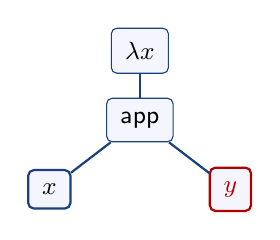
\begin{tikzpicture}[ast,sibling distance=2.3cm,level distance=.88cm]
\node {$\lambda x$} child {node {$\mathsf{app}$}
 child {node {$x$}}
 child {node[draw=red!70!black,text=red!70!black] {$y$}}};
\end{tikzpicture}
\end{column}
\begin{column}{.48\textwidth}\centering
\textbf{After}\\[.7em]
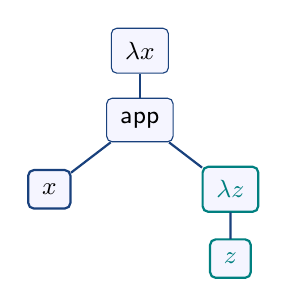
\begin{tikzpicture}[ast,sibling distance=2.3cm,level distance=.88cm]
\node {$\lambda x$} child {node {$\mathsf{app}$}
 child {node {$x$}}
 child {node[draw=teal,text=teal] {$\lambda z$} child {node[draw=teal,text=teal] {$z$}}}};
\end{tikzpicture}
\end{column}
\end{columns}
\vfill
\texttt{t0erm\_subst0(M, "y", T0Mlam("z", T0Mvar("z")))}\\[.5em]
The result is $\lambda x.x\,(\lambda z.z)$. The size increases from $4$ to $5$.
\end{frame}

\begin{frame}[fragile]{Structural recursion: counting nodes}
\begin{lstlisting}
def t0erm_size(term: t0erm) -> sint:
    if False:
        return 0
    elif isinstance(term, T0Mvar):
        return 1
    elif isinstance(term, T0Mlam):
        return 1 + t0erm_size(term.arg2)
    elif isinstance(term, T0Mapp):
        return 1 + t0erm_size(term.arg1) + t0erm_size(term.arg2)
    else:
        raise TypeError(f"t0erm_size({term})")
\end{lstlisting}
Every constructor contributes one node. Recursive calls visit its children.\\[0.5em]
The initial \texttt{if False} branch never runs. It lets every real case use \texttt{elif}.
\end{frame}

\begin{frame}{Size counts constructors, including variable occurrences}
\begin{align*}
\sz(x) &= 1\\
\sz(\lambda x.M) &= 1 + \sz(M)\\
\sz(M\,N) &= 1 + \sz(M) + \sz(N)
\end{align*}
\begin{center}
\begin{tabular}{lrrrr}\toprule
Term & Lambdas & Applications & Variables & Total\\\midrule
$I$ & 1 & 0 & 1 & 2\\
$K$ & 2 & 0 & 1 & 3\\
$S$ & 3 & 3 & 4 & 10\\\bottomrule
\end{tabular}
\end{center}
\medskip
A binder name is a field of a lambda node, so it adds no separate node.\\
Repeated occurrences of a variable each contribute one.
\end{frame}

\begin{frame}[fragile]{Free variables follow the same recursive structure}
\begin{lstlisting}
type fvset = frozenset[strn]

def t0erm_fvset(term: t0erm) -> fvset:
    if False:
        return frozenset()
    elif isinstance(term, T0Mvar):
        return frozenset([term.arg1])
    elif isinstance(term, T0Mlam):
        return t0erm_fvset(term.arg2) - {term.arg1}
    elif isinstance(term, T0Mapp):
        return (t0erm_fvset(term.arg1) | t0erm_fvset(term.arg2))
    else:
        raise TypeError(f"t0erm_fvset({term})")
\end{lstlisting}
\texttt{frozenset} is immutable. Set difference removes the binder name.\\
Set union combines names and removes duplicates.
\end{frame}

\begin{frame}{A free-variable calculation}
\begin{align*}
\FV(\lambda x.x\,y)
 &= \FV(x\,y)\setminus\{x\}\\
 &= (\FV(x)\cup\FV(y))\setminus\{x\}\\
 &= (\{x\}\cup\{y\})\setminus\{x\}\\
 &= \{y\}
\end{align*}
A term is \alert{closed} when its free-variable set is empty.
\[
\FV(I)=\FV(K)=\FV(S)=\varnothing
\]
In Python, the empty result prints as \texttt{frozenset()}.
\end{frame}

\begin{frame}[fragile]{Substitution replaces free occurrences}
\[
M[x:=N]\qquad\text{is represented by}\qquad
\texttt{t0erm\_subst0(M, x, N)}
\]
\begin{lstlisting}
def t0erm_subst0\
(term: t0erm, x0: tvar, tsub: t0erm) -> t0erm:
    def subst0(term: t0erm) -> t0erm:
        # Case analysis on term ...
        ...
    return subst0(term)
\end{lstlisting}
\begin{itemize}
\item \texttt{x0} is the variable name to replace.
\item \texttt{tsub} is the replacement term, assumed to be closed.
\item The nested helper remembers \texttt{x0} and \texttt{tsub} through a Python closure.
\end{itemize}
The excerpt abbreviates the helper body. The next slide shows its cases.
\end{frame}

\begin{frame}[fragile]{The substitution cases}
\begin{lstlisting}
# Inside subst0, after the unreachable if False branch:
elif isinstance(term, T0Mvar):
    return tsub if x0 == term.arg1 else term
elif isinstance(term, T0Mlam):
    x1 = term.arg1
    if x0 == x1:
        return term
    else:
        return T0Mlam(x1, subst0(term.arg2))
elif isinstance(term, T0Mapp):
    return T0Mapp(subst0(term.arg1), subst0(term.arg2))
else:
    raise TypeError(f"subst0({term})")
\end{lstlisting}
A lambda binding \texttt{x0} stops substitution in its entire body.\\
Other lambdas and applications rebuild their nodes using recursive results.
\end{frame}

\begin{frame}{Substitution and shadowing}
Let $I=\lambda z.z$, a closed replacement term.
\begin{align*}
(x\,y)[x:=I] &= I\,y\\[0.5em]
(\lambda y.x\,y)[x:=I] &= \lambda y.I\,y\\[0.5em]
(\lambda x.x\,y)[x:=I] &= \lambda x.x\,y
\end{align*}
In the last example, the lambda binds $x$. There is no free $x$ to replace.\\[1em]
The code returns existing objects for a matching binder and for an unchanged variable. It does not mutate the input term.
\end{frame}

\begin{frame}{Why the replacement must be closed}
Suppose we ignore the assumption and substitute the open term $y$:
\[
(\lambda y.x)[x:=y]
\]
The current function produces $\lambda y.y$. The formerly free $y$ becomes bound: \alert{variable capture}.
\medskip

Capture-avoiding substitution first renames the binder to a fresh name:
\[
\lambda y.x\ \equiv_{\alpha}\ \lambda z.x,
\qquad (\lambda z.x)[x:=y]=\lambda z.y
\]
A closed replacement has no free variables for surrounding binders to capture.\\[0.7em]
\texttt{t0erm\_subst0} assumes this precondition but does not check it.
\end{frame}

\begin{frame}{What the program does when run}
\begin{itemize}
\item Defines the syntax classes and constructs \texttt{EX\_I}, \texttt{EX\_K}, and \texttt{EX\_S}.
\item Prints each example using its data-class representation.
\item Prints sizes $2$, $3$, and $10$, followed by three empty free-variable sets.
\item Defines substitution, but includes no substitution calls at the top level.
\end{itemize}
\medskip
The top-level print statements also execute when the module is first imported.\\[0.8em]
An evaluator could use substitution for a beta step:
\[
(\lambda x.M)\,N \longrightarrow_{\beta} M[x:=N]
\]
The file has no evaluator yet. Its substitution function requires closed $N$.
\end{frame}

\begin{frame}[fragile]{Practice: predicting the results}
\begin{lstlisting}
M = T0Mlam("x",
        T0Mapp(T0Mvar("x"), T0Mvar("y")))

# Predict:
t0erm_size(M)
t0erm_fvset(M)
t0erm_subst0(M, "y", EX_I)
t0erm_subst0(M, "x", EX_I)
\end{lstlisting}
\pause
\medskip
\textbf{Answers:} $4$, $\{y\}$, $\lambda x.x\,(\lambda x.x)$, and $M$.\\[0.6em]
In the third answer, the inner $\lambda x$ binds only its own body.\\
The inserted identity remains closed even though its binder has the same name.
\end{frame}
\end{document}
